\documentclass[a4paper]{article}
\usepackage{amsmath}
\usepackage{amssymb}
\usepackage{fancyhdr}
\usepackage{a4wide}
\usepackage{geometry}
\usepackage[utf8]{inputenc}
\geometry{a4paper,left=2cm,right=2cm, top=3cm, bottom=3cm}
\usepackage{listings}
\usepackage{graphicx}

\newcommand{\titel}[1]{\fancyhead[C]{#1}}
\newcommand{\name}{\fancyhead[L]{Alexander Landmesser}}
\newcommand{\matrikel}{\fancyhead[R]{Matrikelnummer: 1096552}}
\newcommand{\pl}{\hspace*{1cm}}
\begin{document}
\title{Algorithm Engineering}
\maketitle
\section*{Datentypen}

\subsubsection*{Getränkeautomat}
Automat akzeptiert 1E, ein Getränk kostet 3E\\
Operatoren:
\begin{enumerate}
\item Init(Reset)
\item Akzeptiere1E
\end{enumerate}
Init $\rightarrow$ Zustand\\
\hspace*{0.5cm}Semantik: Automat geht in Zustand 0\\
Akzeptiere1E: ZustandX\{0,1\} $\rightarrow$ ZustandX\{tue nichts, gib Getänk\}\\
\hspace*{0.5cm}Semantik: Beschreibung durch einen endlichen Automaten.
\subsubsection*{Stadtplan}
Übung 1
\subsection*{Bemerkungen}
\begin{itemize}
\item Operatoren können partiell Definiert sein. Man gibt Definitionsbereich oft in einer Vorbedingung an.
\item Operatoren, bei denen der Datentyp selbst auf der linken Seite nicht vorkommt, heißen \underline{Konstruktoren}. Sie erzeugen ein neues Objekt (bzw. versetzen den Typ in einem bestimmten Zustand).
	\begin{itemize}
		\item Create: $\rightarrow$ stack$<$T$>$
		\item Create: int $\rightarrow$ vector (Vektor bestimmter Dimension)
	\end{itemize}
\item Objekt- und Zustandssicht sind beide nützlich. \underline{Stack/Getränkeautomat} haben internen Zustand, Operatoren können ihn verändern.
	\begin{itemize}
		\item Integer: Objektsicht besser, Operatoren erzeugen neue Objekte, exisitierende werden nicht geändert.
	\end{itemize}
\item stack$<T>$ ist ein parametrisierbarer Datentyp: Stack mit Elementen vom Typ T. Hat eventuell besondere Anforederungen an Typ T, z.B. $x\leq y$ in Dictionaries.
\item Man kann nun eigentlich schon programmieren, obwohl über die Interpretiernug noch nichts bekannt ist.

\end{itemize}
\subsubsection*{Anwendung von stack$<T>$}
Auswertung von Postfix-Ausdrücken\\
Vereinfachungen: alle Operatoren binär (+-*/), Eingabe nur Zahlen 0-9\\
\underline{Bsp.:} $(7-5)*(3+1)\rightarrow 75-31+*$
\subsection*{Defintion eines Datentyps}
(In einer Objekt-Orientierten Programmiersprache)\\
\begin{lstlisting}[language=c++]
class Typname {
	//Definition der Menge der Objekte bzw Zustaende
	private: //Deklaration von Variablen zur Darstellung der Objekte/Zustaende
	public: //Operatoren
	//Kommentare z.B. ueber Effizienz
};
\end{lstlisting}
\subsubsection*{Operatoren}
Methoden/Memberfunktionen\\
Syntax: Ergebnistyp Name(Argumente...);\\
\underline{Spezielle Methoden:} 
\begin{itemize}
	\item Kein Ergebnistyp: stack(); stack(size);
	\item Destruktor: $\sim$ Typname();
\end{itemize}
\subsection*{Beispiel}
int\_stack $\rightarrow$ stack$<T>$\\
\begin{lstlisting}[language=c++]
class int_stack {
	/* Eine Instanz vom Typ int_stack ist eine Folge von ganzen Zahlen (int). Eine Folge der laenge 0 heisst der leere Stack.*/
	private: //Implementierung
	public: stack(int sz); //Konstruktor
	//Erzeugt einen Stack mit maximaler Groesse sz
	~stack() //Destruktor
	void push (int x);
	//fuegt x als letzes Element (top) an die Folge an.
	int top() const;
	//liefert das letzte (top) Element
	//Precondition: Stack nicht leer
	int pop();
	//entfernt letztes (top) Element der Folge und gibt es zurueck
	//Precondition: Stack nicht leer
	bool empty() const;
	//true, wenn Stack leer, false sonst.
	
\end{lstlisting}
In c++ Spezielle Header Datei, die die Deklarationen ohne Rumpf enthält. Implementierung in .cpp\\
\subsubsection*{Implementierung der Klasse int\_stack}
Mehrere Möglichkeiten: Array, Liste
Array Implementierung:
$int_stack.h$
\begin{lstlisting}
class int_stack {
	private 
		int* A; //Feld
		int sz; //Laenge von A
		int t;
};
\end{lstlisting}
$int_stack.cpp$
\begin{lstlisting}[escapechar=!]
#include "int_stack.h"
int_stack::int_stack(int n) {
	sz=2;
	A = new int[sz];
	t = -1; //leer
}
int_stack::~int_stack(){
	delete[] A;
}
void int_stack::push(int x){
	if (t == sz-1){
		//stack voll
		int* B=new int[2*sz];
		sz !$\leftarrow$! 2*sz;
		for(int i=0; i !$\leq $!;i++){
			B[i] !$\leftarrow $!
		}
		delete[] A;
	}
	A[++t] !$\leftarrow $! x; //eigentlich push
}
int int_stack::pop(){
	if(t==-1){
		EXCEPTION("Leerer Stack")
	return A[t--];
}

\end{lstlisting}
\subsubsection*{Einschub: Variablen, Konstruktoren, Wertzuweisung}
%TODO Einrückung!
\begin{itemize}
\item[Variablen Deklaration] c++: Aufruf des Konstruktors generiert ein Objekt.\\
	Java: Erst eine Referenz erstellen, dann ein Objekt generieren und auf dieses verweisen.
\item[Wertzuweisung] c++: $int_stack s1,s2; s1=s2;$ Objekt wird kopiert, es gibt 2 Objekte.\\
	Java: $int_stack s1,s1; s1=s2;$ Referenzen zeigen auf ein einziges Objekt.
\item[Referenzsemantik in c++:] Verwendet Pointer auf ein Objekt.\\
	Test auf Gleichheit (==) Operator\\
	Parameterübergabe sind Pointer
\item[Referenzsemantik in Java:] Parameter by Value, gesamtes Objekt kopiert und dann übergeben.
\end{itemize}
\subsection*{Korrektheit einer Implementierung}
(Hier der Array-Implementierung von $int_stack$)\\
Eigentlich 2 Datentypen:
\begin{itemize}
\item[1.] der abstrake Datentyp $int_stack$
\item[2.] der konkrete Datentyp Array
\end{itemize}
\underline{Abstrakter Zustand:} Folge von int's\\
\underline{Konkreter Zustand:} Werte der Variable A,t,sz\\
Wir garantieren (Invariante), dass nicht die Kombination von A,t,sz möglich sind, sondern nur gültige Zustande mit:
\begin{itemize}
\item[1.]A ist ein Feld der Länge sz
\item[2.] $-1 \leq t\leq sz-1$
\end{itemize}
Sei Z=Menge der konkreten Zustände und S = Menge der abstrakten Zustände\\
Um die Korrektheit zu zeigen, definieren wir eine Abbildung $F: Z \rightarrow S$\\
$(A,sz,t) \rightarrow \left\lbrace \begin{array}{l}
	Folge\ A[0],...,A[t]\ falls t\geq 0\\
	Leere\ Folge, t=-1
\end{array}\right.$
Und zeigen:
\begin{itemize}
\item[1.] Konstruktoren erzeugen gültige konkrete Zustände
\item[2.] Für jede abstrakte Operation und die dazugehörige konkrete Operation $f_{op}$ zeige $F(f_{op}(Z)) = op(F(Z))$
	Bsp.: push: $S\times int \rightarrow S $\\
	$f_{push}: Z \times int \rightarrow Z$
\end{itemize}
Kommutatives Diagramm:\\
$z \xrightarrow{F} s$\\
$\downarrow f_{op} \uparrow op$\\
$z' \xrightarrow{F} s'$
\subsection*{Vererbung/Generische Datentypen}
Templates/Wiederverwendung von Code\\
\underline{Situation}\\
Man braucht einen Datentyp A, der sehr ähnlich zu einem bereits vorhandenen definierten Typ B ist.\\
A soll:\\
\begin{itemize}
\item einen Teil der Daten/Operationen verwenden
\item andere Daten/Operationen anfügen
\item einige verändern (auf andere Weise implementieren)
\end{itemize}
\subsubsection*{Beispiel}
Es existiert die Klasse Polygon (B), implementiert werden soll eine Klasse Rechteck (A).\\
A ist eine Spezialisierung von B\\
Rechteck könnte alle Polygon-Operationen (draw(),translte etc)\\
Einige Operationen können effizienter implementiert werden (Flächeninhalt etc.)\\
Andere sind nur für Rechtecke definiert.\\
Jedes Rechteck ist ein spezielles Polygon.
\subsubsection*{Allgemein}
Wir leiten die Klasse A von der Klasse B ab.\\
Syntax in c++: A: public B\\
\begin{lstlisting}
class Rechteck: public Polygon{
	//Konstruktoren -> uebung :(
	private:
		//Ueberschreiben
		double b,h;
		double area() {return b*h;}
		double umfang() {return 2*(b+h);}
		//Hinzufuegen
		double ratio() {return b/h;}
};
\end{lstlisting}
Ableitungen auch als Baum darstellbar (Shape mit Kindern Polygon/Ellipse/Punkt etc)\\
\subsubsection*{Typverträglichkeit}
Einer Variable vom Typ B* oder B\& (alle Variablen in JAVA vom Typ B) kann ein Opbjekt (Pointer/Referenz) vom Typ A zugewiesen werden.\\
Alle im Ableitungsbaum erreichbaren Typen können zugewiesen werden (Kinder).\\
Eine Variable hat 2 Typen: Einen Statischen Typ, der zur Compilezeit bekannt ist. Dynamischer Typ, der zur Laufzeit bekannt ist.
\subsection*{Polymorphe Datenstrukturen}
\begin{lstlisting}
polygon* p = new rechteck()
double func(polygon& p){
	return poly.area();}
rechteck rect = new rechteck();
func(rect);
\end{lstlisting}
Es wird per dynamischer Bindung die Funktion func der Klasse Rechteck aufgerufen.\\
C++ benutzt standardmäßig statische Bindung esseidenn Funktion ist "virtual".
Bsp.: Feld von Polygonen\\
c++: Polygon** (Ein Pointer auf ein Feld von Pointern) A = new Polygon*[100];\\
A[0] = new Polygon(...);\\
A[1] = new Rechteck(...);\\
\\
Abstrakte Klassen werden verwendet um Interfaces zu definieren.\\
Z.B. Shape als abstrakte Klasse. In C++ werden Methoden als abstrakt markiert, wenn sie bei der Deklaration = 0 gesetzt werden\\
virtual void draw() = 0;\\
\subsection*{Anwendung auf Algorithmen}
Lineare Ordnungen durch ein Interface umgesetzt.\\
In C++:\\
\begin{lstlisting}
class comparable{
	virtual int compare(compareable x)=0;
}
\end{lstlisting}
Anwendung in generischen Sortieralgorithmen:\\
Quicksort(comparable* A[])\\
Zum Vergleich benutzt man x.compare(y)\\
\subsubsection*{Anwendung: Sortiere ein Feld von point}
\begin{lstlisting}
class point: public comparable{
	int compare(comparable x){
		//x ist tatsaechlich ein point
		double px=((point&)p).x; //Casting
		double py=((point&)p).y;
		//lexikographische Ordnung..
		return ..;
	}
}
Aufruf von Quicksort:
point* A[] = new point*[100];
for(i=0;i<100<i++) A[i] = new point(i,i*i);
Quicksort(A,100);
\end{lstlisting}
Datenstrukturen, bei denen Comparable sinnvoll ist:\\
\begin{itemize}
\item Binäre Suchbäume, bei denen die Knoten vergleichbar sind.
\end{itemize}
\subsubsection*{Weitere Anwendung von Vererbung}
Generische Datenstrukturen wie z.B. Listen von beliebigen Objekten.\\
Einfach verkettete Liste:\\
Beobachtung: Implementierung der Operationen (push, pop), ist nicht abhängig vom Typ. Der Wert (int,string,point,...) jedoch schon.\\
Abstraktion: Liste ohne Werte\\
1. Basisklasse für allgemeines Listenelement:
\begin{lstlisting}
class slist_element{
	slist_element* next;
	slist_element(slist_element* p) {next = p;}
};
\end{lstlisting}
2. Basisklasse für allgemeine List:
\begin{lstlisting}
class slist{
	slist_element* first;
	slist() {first = NULL;}
	
	void push(slist_element* p){
		p->next = first;
		first = p;
	}
	slist_element* pop(){
		if(first == NULL) return first;
		slist_element* p = first;
		first = first.next;
		return p;	
	}
}
\end{lstlisting}
slist funktionirt auch für alle von slist\_elem abgeleiteten Klassen.\\
Besondere Elemente werden als neue Klassen definiert, die von slist\_element erben.\\
Ein "Point" ist ein "slist\_element"\\
\begin{lstlisting}
slist L;
point* p = new point(x,y);
L.push(p);
\end{lstlisting}
slist ist Polymorph, es kann als Liste verschiedener Datentypen dienen.\\
Situationen in denen diese Polymorphie vorteilhaft ist: Grafik-Editor:\\
\begin{lstlisting}
void drawAll() //Iteriere ueber Liste und rufe draw fuer alle auf
forall x in scene //scene ist die Liste
	x -> draw();
\end{lstlisting}
Falls wir eine Liste von einem bestimmten Objekt-Typ verwenden wollen (z.B.b point\_list) wird diese von slist abgeleitet.\\
\begin{lstlisting}
class point_list: public slist {
	//neues Interface das nur points erlaubt
	void push(point* p) {slist::push(p);}
	point* pop(){return (point*) slist::pop();}
	//Das Casting ist sicher, da durch push sicher nur points in der Liste sind.
}
\end{lstlisting}
Aufwändige Datenstruktur: Balancierte Suchbäume (z.B. AVL)\\
1. Klasse für die Knoten (benötigt parent, left, right)
\begin{lstlisting}
class bin_tree_node{
	bin_tree_node* left, right, parent;
};
\end{lstlisting}
2. Klasse für den Baum:
\begin{lstlisting}
class bin_tree{
	virtual int cmp(bin_tree_node* p, bin_tree_node* u) = 0
	//Bsp.: cmp(p,q) = {-1, wenn p<q; 0, wenn p = q; 1, wenn p>q}
	void insert(bin_tree_node* p){
		//fuegt p in den Baum ein, verwendet cmp als Vergleich	
	}
	bin_tree_node* lookup(bin_tree_node* p){
		/* in Schleife: 
		if cmp(q,p) > 0 q=q->left;
			else q=q->right;
			*/
	}
}
\end{lstlisting}
Anwendung auf Point: 
\begin{lstlisting}
class point:public bin_tree_node{
	...
}
class point_bin_tree:public bin_tree{
	//Definiere cmp Funktion
	int cmp(bin_tree_node* p, bin_tree_node* q){
		point* a = (point*)p;
		point* b = (point*)q;
		if(a->x < b->x) return -1;
		if(a->x > b->x) return 1;
		if(a->y < b->y) return -1;
		if(a->y > b->y) return 1;
		return 0;	
	}
	void insert(point* p){
		bin_tree::insert(p);
	}
	point* min() {return (point*)bin_tree::min();}	
}
\end{lstlisting}
\section*{Templates}
\subsection*{Funktionstemplates}
\textit{template $<$class T$>$}\\
Beispiel: swap(T\& x, T\& y) Vertauscht den Inhalt der beiden Variablen\\
\begin{lstlisting}
 swap(T& x, T& y){
 	T tmp = x;
 	x = y;
 	y= tmp;
 }
\end{lstlisting}
Implementierung ist unabhängig von T.
\subsection*{Klassentemplates}
\begin{lstlisting}
template<class T>
class stack{
	T* A; //Feld von T's
	int sz;
	int t;
	
	public
	void push(T x){...}
	T pop {...}
}
\end{lstlisting}
Beispiel für mehrere Typen:
\begin{lstlisting}
template<class K, class I>
class dictionary{
	//Woerterbuch mit Schluessel vom Typ K und werte vom Typ I
	void insert(K k,I i){...}
	I translate (K key){...}
}
\end{lstlisting}
Anwendungsbeispiel: Word-Count, zählt wie oft einzelne Wörter in einem Text vorkommen.
dictionary$<$string,int$?>$ D; Speichert Wort als Schlüssel, Häufigkeit als Wert.
\section*{Fortgeschrittene Datenstrukturen und Algorithmen}
LEDA: Library of Efficient Datatypes and Algorithms\\
Plattform: Algorithmus $\rightarrow$ Programm\\
Datentypen:  Listen, Stacks, Dictionaries, Priority Queue\\
Efficient: Datenstrukturen\\
Einfache Benutzung (Pseudocode soll leicht in C++ umsetzbar sein)\\
Korrektheit: Datentypen (Definition), Program Checker\\
Weitere Themen: Graph-Datenbanken, -Algorithmen, Geometrie\\
\subsection*{Spezifikationen von Datentypen in LEDA}
Item-Konzept: Viele Datentypen sind Definiert als Menge von Items.\\
Item: Zugriff über Parameter (Abstraktion von den Begriffen Pointer, Referenz, Index)\\
Bsp.: dictionary$<string, int>$ D speichert Paare aus Schlüsseln (string) und Informationen (int)\\
Definition: D ist eine Menge von Items (dictionary-Items)\\
Operationen: \\
\begin{itemize}
\item D.insert(string s, int i): Falls D kein Item mit Schlüssel s enthält, füge Item (s,i) ein und gib es zurück. Sonst: Ändere Datenwert i und liefere es zurück.
\item D.lookup(strin s): liefet das Item mit dem Schlüssel s, falls es nicht existiert, Null.
\end{itemize}
2. Beispiel: Priority Queue\\
$priority\_queue<P,I> PQ$\\
P: Priorität z.B. Zahl, I: Information (z.B. Knoten eines Graphen)\\
Definition: Menge von Items\\
Operationen: insert, findMin (minimale Priorität), prio (setze Priorität), inf (setze Information), delmin, decrease\_P\\
\subsection*{Dijkstra Algorithmus}
Eingabe: Graph $G=(V,E)$, Kostenfunktion $cost=E\rightarrow int^+$, Startknoten $s\in V$\\
Ausgabe: Distanzfunktion $dist:V\rightarrow int^+$, dist(v) = Kosten eines billigsten Pfades von s nach v.\\
\hspace*{1cm}Kosten eines Pfades: Summe der Kanten.\\
Idee von Dijkstra:\\
\begin{itemize}
\item Überschätze Distanzfunktion: 0, falls s=v, $\inf$, falls $s\neq v$.
\item Kandidatenlist U: Menge aller Knoten, aus deren Kanten ausgehen können, die eine Abkürzung darstellen.
\item Wähle jeweils $u\in U$ mit dist(u) minimal
\item Beobachtung: dist(a) ist korrekt.
\item Durchlaufe alle aus u ausgehenden Kanten und überprüfe Dreiecksungleichung, reduziere Distanz von v
\end{itemize}
Kann effizient mit Fibonacci Heap realisiert werden.
\subsection*{Graphalgorithmen in LEDA}
\subsubsection*{Der Datentyp Graph}
Dient zur Erstellung von gerichteten Graphen G=(V,E) mit $E \subseteq (V \times V)$\\
\subsubsection*{Arten von Objekten}
Operationen auf einem Graphen G:\\
Access Operationen:\\
\hspace*{1cm}node G.source(Edge e): Von welchem Knoten geht die Kante e aus\\
\hspace*{1cm}node G.target(Edge e): Zu welchem Knoten geht die Kante e\\
\hspace*{1cm}int G.outdeg(node v): Ausgangsgrad\\
\hspace*{1cm}int G.indeg(node v): Eingangsgrad\\
\hspace*{1cm}list\textless edge\textgreater G.out\_edges(node v)\\
Update Operationen:\\
\hspace*{1cm}node G.new\_node()\\
\hspace*{1cm}edje G.new\_edge(node v, node w)\\
\hspace*{1cm}void G.del\_edge(edge e)\\
\hspace*{1cm}void G.del\_node(node v) (entfernt v und alle Kanten)\\
Iterationen (Laufvariable wird extern deklariert, weil weil):\\
\hspace*{1cm}forall\_nodes(v,G)\\
\hspace*{1cm}forall\_edges(e,G)\\
\hspace*{1cm}forall\_out\_edges(e,v)\\
\hspace*{1cm}forall\_in\_edges(e,v)\\
Beispiel: Iteration über alle Nachbarknoten von v:\\
\begin{lstlisting}
forall_out_edges(e,v){
	node w = G.target(e)
}
\end{lstlisting}
Beispiel: Teste, ob G azyklisch\\
Idee: Siehe topologisches Sortieren: \\
\hspace*{1cm}Solange ein Knoten v existiert mit indeg(v)=0, entferne ihn und alle ausgehenden Kanten.\\
\hspace*{1cm}Falls G leer, dann ist der Graph azyklisch.
\begin{lstlisting}[escapechar=!]
zero <- {v !$\in$! V | indeg(v) = 0}
while zero !$\neq \emptyset$! do
	u <- beliebiger Knoten aus zero
	zero <- zero\{u}
	forall v !$\in$! V mit (u,v) !$\in$! E
		entferne (u,v) aus G
		if indeg(v)=0 then
			zero <- zero !$\cup$!{u}
		fi
	od
	entferne u aus G
od
\end{lstlisting}
Als C++ Programm (oder auch nicht... Näherliegende Gründe):
\begin{lstlisting}
bool isAcyclic (graph G) //Call by Value, Graph wird kopiert
	stack<node> zero;
	node v;
	forall_nodes(v,G){
		if (G.indeg(v)==0) zero.push(v);
	}
	while (!zero.empty()){
		node u = zero.pop();
		edge e;
		forall_out_edges(e,u){
			node v = G.target(e);
			G.del_edge(e);
			if (G.indeg(v)==0) zero.push(v);
		}
	}
	return G.number_of_edges()==0;
}
\end{lstlisting}
Informationen (Daten) mit den Knoten und Kanten speichern.\\
\subsubsection*{Parametrisierter Graph}
Netzwerk: Knoten stehen für Objekte vom Typ vtype, Kanten etype.\\
Unterklasse vom gegebenen graph\\
$GRAPH<vtype,etype> G$;
\subsubsection*{Node/Edge Array}
$node\_array<T> A(G)$ Mit G einem Graph\\
$edge\_array<T> B(G)$\\
Z.B. Kürzester Weg: DIJKSTRA(graph G, $edge\_array<int>$ cost,node startNode, $node\_array<int>$ distance);\\
Einige Ausgabedaten werden getrennt vom Graphen übergeben.\\
\subsection*{Erstes konkretes Beispiel: Dijkstra}
\begin{lstlisting}
void DIJKSTRA (graph& G, node s, edge_array<int>& cost, node_array<int>& dist)
{
	p_queue<node,int> PQ;
	node_array<pq_item> I(G);
	dist[s] = 0;
	I[s] = PQ.insert(s,0);
	node v;
	forall_nodes(v,G){
		if(v!=s) dist[s] = MAXINT;
	}
	While (!PQ.empty()){
		node u = PQ.delmin();
		edge e;
		forall_out_edges(e,u){
			node w = G.target(e);
			int d = dist[u]+cost[e];
			if(d<dist[w]){	//Dreiecksungleichung
				if(dist[w]==MAXINT) //Wurde schon besucht?
					I[w] = PQ.insert(w,d)
				else PQ.decrease_p(I[w],d)
				dist[w] = d;
		}
	}		
\end{lstlisting}
Analyse: delmin, insert wird n mal ausgeführt. decrease\_p wird m mal (für alle nodes und alle deren Kanten) asugeführt.\\
Ergebnis: O((m+n)log n)\\
Korrektheit:\\
Idee: Füge Programmcode hinzu, der für eine konkrete Testeingabe überprüft, ob das Ergebnis korrekt ist.\\
Teste am Ende, ob für jede Kante die Dreiecksungleichung erfüllt ist.
\begin{lstlisting}
edge e;
forall_edges(e,G){
	node v = G.source(e);
	node w = G.target(e);
	ASSERT(dist[v] + cost[e] >= dist[w]);
}
\end{lstlisting}
\subsection*{Netzwerkflussprobleme: Maxflow }
Graph: Transportnetzwerk \\
Jede Kante besitzt eine Kapazität (wie viel pro Zeiteinheit über diese Kante transportiert werden kann).\\
\underline{Probleme:}
\begin{itemize}
\item[1. ]Maximiere den Transport von einem Knoten s (Source) zu einem Knoten t (Senke)
\item[2. ]Minimiere die Transportkosten (min cost flow)
\end{itemize} 
Eingabe: Graph $G=(V,E)$, Knoten $s, t \in V | s\neq t$, Kapazitäten $u\rightarrow \mathbb{R}^+_0$\\
Schreibweise: $u_{ij}$ für $(u: u(i,j))$\\
Ergebnis: Flussfunktion $x: E \rightarrow \mathbb{R}^+_0$ mit:
\begin{itemize}
\item[1. ]$\forall (i,j) \in E: 0\leq x_{i,j} \leq u_{i,j}$ Kapazitätsbedingung
\item[2. ]$\forall i\in V \backslash \{s,t\}: \sum_{j\in V mit (i,j)\in E} x_{i,j} = \sum_{k\in V | (k,i)\in E} x_{k,i}$ (Die Menge, die aus i rausgeht, muss auch in i reinkommen).
\end{itemize}
Gesucht ist ein Fluss x mit $\sum_{i\in V | (s,i)\in V} x_{s,i} - \sum_{j\in V | (j,s)\in V} x_{js}$ maximal.\\
$\forall i\in V \backslash \{s,t\}  \delta (i)=0$ maximiere $\delta (s)$\\
Beobachtung: $\delta (t) =-\delta (s)$\\
\subsubsection*{Idee für einen Algorithmus: Erhöhende Pfade}
\begin{itemize}
\item Starte mit allen x=0 $(\forall (i,j) \in E: x_{i,j} \leftarrow 0)$
\item Erhöhe x entlang von Pfaden von s nach t.
\end{itemize}
\underline{Definition} Restnetzwerk G(x) (hängt vom aktuellen Fluss x ab), beschreibt die Möglichkeiten x zu verändern.\\
\underline{Erhöhende Pfade} Pfad P von s nach t in G(x). Erhöung von $\delta = min \{ r_{i,j} | (i,j)\in P\}$\\
\underline{Achtung} Der reale Pfad in G hat eventuell Kanten in Gegenrichtung.
\underline{Beispiel:}\\
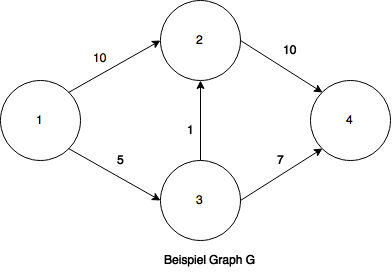
\includegraphics[scale=0.4]{AE10.png}
\begin{itemize}
\item[1.] $x\leftarrow 0, G(x)=G$ (man lässt sonst alle Kanten mit Kapazität 0 weg)
\item[2.] Pfad $s\rightarrow t$ suchen, z.B. $a\rightarrow^5 3 \rightarrow^1 2 \rightarrow^{10} 4$
\item[3.] Pfaderhöhung um $\delta$. $\delta = 1$, da minimale Kapazität = 1\\ 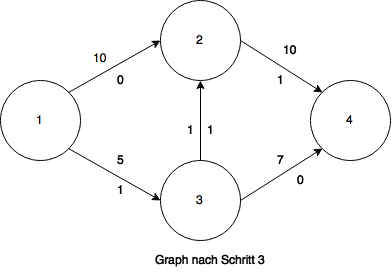
\includegraphics[scale=0.3]{AE10-2.png}
\item[4.] Bestimmmung des neuen G(x) (Restkapazitäten)\\ 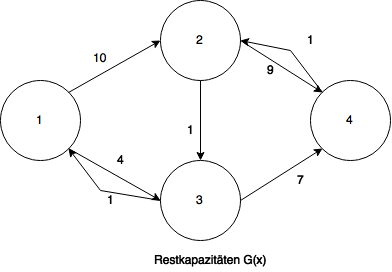
\includegraphics[scale=0.3]{AE10-3.png}
\end{itemize}
%%BLATT HIER REIN 
\underline{Korrektheit} x ist immer ein Fluss. Terminiert mit Fluss x, sodass in G(x) kein Pfad von s nach t (bitte was?)
\underline{Implementierung} 
\begin{itemize}
\item[1] Keine explizite Darstellung von G(x), stattdessen Navigiere im Originalgraphen, verwende ausgehende Kanten, wenn $u_{i,j} > x_{i,j}$, eingehende Kanten, wenn $x_{i,j} > 0$.
\item[2] Berechnung eines erhöhten Pfades: Verwende DFS oder BFS vom Knoten s aus, und berechne die Kanten wie in 1. beschrieben. Stoppe, wenn t erreicht.
\item[3] Darstellung des Pfades durch pred\_Verweise (Vorfahrverweise).
\end{itemize} 
\subsubsection*{Beispiel Pfaderhöhung (MaxFlow)}
Idee: Suche alle im Restnetzwerk erreichbaren Knoten bis t gefunden wurde (mit DFS,BFS o.A.)\\
Algorithmus Labelling:\\
\hspace*{1cm} graph G;edge\_array$<int>$ cap; edge\_array$<int>$ flow;node\_array$<bool>$ label; node\_array$<edge>$ predecessor;\\
\begin{lstlisting}[escapechar=@]
//UEbergabeparameter: Startknoten s
edge e;
forall_edges(e,G) flow[e] @$\leftarrow$@ 0;
node v;
forall_nodes(v,G){
	labelled[v] @$\leftarrow$@ fale;
	pred[v] @$\leftarrow$@ NULL;
}
while(true){
	queue<node> S;
	S.append(s);
	labelled[s] @$\leftarrow$@ true;
	while(S.empty() == false){
		node v = S.pop();
		//iteriere alle im Restnetzwerk adjazenten Kanten
		edge e;
		forall_out_edges(e,V) {
			if(flow[e] == cap[e]) continue;
			node w = G.target(e);
			if(labelled[w]) continue;
			labelled[w] @$\leftarrow$@ true;
			pred[w] @$\leftarrow$@ e;
			S.append(w);
		}
		forall_in_edges(e,V){
			if(flow[e] == 0) continue;
			node w = G.source(e);
			if(labelled[w]) continue;
			labelled[w] @$\leftarrow$@ true;
			pred[w] @$\leftarrow$@ e;
			S.append(w);
		}
	}
	if(labelled[t] == false) break; //t nicht erreichbar
	int delta = MAXINT;
	node v = t;
	while (v != s){
		edge e = pred[v];
		int r = (G.source(e) == v) ? flow[e] : cap[e]-flow[e];
		if(r<delta) delta = r;
		v = (G.source() == v) ? G.target(e) : G.source(e) ;
	}
	v = t;
	while(v!=s){
		edge e = pred[v];
		if(v==G.target(e)){
			flow[e]+=delta;
			v = G.source(e);
		}else{
			flow[e]-=delta;
			v = G.target(e);
		}
	}
		
}
\end{lstlisting}
\subsection*{Geometrische Algorithmen}
In $\mathbb{R}^2$\\
Objekte (Klassen/Typen): Point,segment (Strecken), line (Gerade)\\
Operationen: Vergleiche, Orientierung (Lage eines 3. Punktes zum Strahl zwsichen den ersten beiden)
\subsection*{Grundoperationen}
\textbf{a.orientation(b,c)}\\
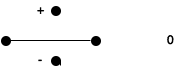
\includegraphics[scale=1]{orientation.png}\\
\textbf{Vergleich von Punkten}\\
a.cmp\_xy(b): +1, wenn $a>_{xy}b$, 0 wenn $a=b$, -1 wenn $a<_{xy}b$\\
\textbf{Min/Max in xy}: trivial\\
\textbf{Vergleich von Entfernungen}\\
Ist c oder b näher an a...\\
$sign((d_x^2+d_y^2) - (d_x^{'2} + d_y^{'2}))$ \\
Bei allen Grundoperationen muss nur +,- und * verwendet werden, schneller und exakt\\
\subsection*{Anwendung von orientation}
Strecke: segment(a,b)\\
point s.start(), point s.end()\\
\textbf{Schnitt von zwei Segmenten:} \\
Zwei Segmente (a,b) (c,d): a,orientation(b,c) != a.orientation(b,d) $\wedge$ c.orientation(d,a) != c.orientation(d,b)\\
\subsection*{Konvexe Hülle}
\textbf{Eingabe:} Liste von Punkten L\\
\textbf{Ausgabe:} Kleinstes konvexes Polygon P, das alle Punkte enthält (Polygonecken sind Punkte aus L)\\
\textbf{Konvex:} Alle Winkel des Polygons $>$ 180 Grad, jede Strecke zwischen zwei Punkten in diesem Polygon liegt komplett im Polygon.\\
\textbf{Ausgabe:} Ecken gegen den Urzeigersinn sortiert (und nummeriert)\\
\textbf{Algorithmus:} Gift wrapping (Ursprünglich im Raum)\\
\hspace*{1cm} Starte bei $Min_{xy}(L)$\\
\begin{lstlisting}
list<point> convexHull(list<point> &L){
	list<point> P;
	point q0 = L.first();
	point p;
	forall(p in L){
		if(p.cmp_xy(q)  == -1) q0=p;
	}
	P.append(q0); L.del(q0);
	while 1{
		point q = L.first()
		forall(p in L){
			if P.last().orientation(q,p) == -1 ||
			(P.last().orientation(q,p) == 0 && P.last().cmp_dist(q,p) == -1)
				q = p;
		}
		L.del(q);
		if q==q0 break
		else P.append(q);
	}
	return P;
			
\end{lstlisting}
\end{document}
